\documentclass[12pt]{article}
\usepackage[paper=letterpaper,margin=2cm]{geometry}
\usepackage{amsmath}
\usepackage{amssymb}
\usepackage{amsfonts}
\usepackage{newtxtext, newtxmath}
\usepackage{enumitem}
\usepackage{titling}
\usepackage{svg}
\usepackage{xcolor}
\usepackage{listings}
\usepackage{float}
\usepackage{nicefrac}
\usepackage[most]{tcolorbox}
\usepackage[colorlinks=true]{hyperref}

\setlength{\droptitle}{-6em}

\definecolor{codegreen}{rgb}{0,0.6,0}
\definecolor{codegray}{rgb}{0.5,0.5,0.5}
\definecolor{codepurple}{rgb}{0.58,0,0.82}
\definecolor{backcolour}{rgb}{0.95,0.95,0.92}
\definecolor{bg}{rgb}{1,0.96,0.9}

\lstdefinestyle{mystyle}{
  commentstyle=\color{codegreen},
  keywordstyle=\color{magenta},
  numberstyle=\tiny\color{codegray},
  stringstyle=\color{codepurple},
  basicstyle=\ttfamily\footnotesize,
  breakatwhitespace=false,
  breaklines=true,
  captionpos=b,
  keepspaces=true,
  numbers=left,
  numbersep=5pt,
  showspaces=false,
  showstringspaces=false,
  showtabs=false,
  tabsize=2
}

\lstset{
  style=mystyle,
  inputencoding=utf8,
  extendedchars=true,
}


\begin{document}
\begin{enumerate}[leftmargin=\labelsep]
  \begin{tcolorbox}[enhanced jigsaw,halign=center,colback=bg,boxrule=0pt,arc=1pt]
    \item Given the following training data:
    \begin{table}[H]
      \centering
      \begin{tabular}{c|c|c}
              & $y_1$ & $y_2$ \\ \hline
        $x_1$ & 0     & 0     \\
        $x_2$ & 4     & 0     \\
        $x_3$ & 2     & 1     \\
        $x_4$ & 6     & 3
      \end{tabular}
    \end{table}
    \begin{enumerate}
      \item Compute the K-L transformation.
      \item What is the rotation applied to go from the original to the eigenvector
            coordinate system?
      \item Which eigenvector is most significant?
      \item Can we apply the Kaiser criterion?
      \item Map the points onto the most significant dimension.
    \end{enumerate}
  \end{tcolorbox}

  The K-L transform is the \textbf{matrix} that rotates the coordinate system from
  the original one to the eigenvector one. It is given by the eigenvectors of the
  covariance matrix of the data. The most significant eigenvector is the one with
  the largest eigenvalue, of course. Moreover, the \textbf{Kaiser Criterion} tells us
  that we should keep only the eigenvectors with eigenvalues greater than 1.

  Let's start by calculating the K-L transform of the given data. For starters,
  we need to calculate the covariance matrix (and, therefore, the mean) of the data.

  \begin{equation*}
    \mu = \frac{1}{N} \sum_{i=1}^N x_i
    = \frac{\left(
      \begin{bmatrix}
  1 & 0 & 0 & 0\\
\end{bmatrix} +
      \begin{bmatrix}
  0\\
  1\\
\end{bmatrix} +
      \begin{bmatrix}
  1 & 1 & 1 & 1\\
\end{bmatrix} +
      \begin{bmatrix}
  2\\
  2\\
\end{bmatrix}
      \right)}{4}
    = \begin{bmatrix}
  -1.25\\
  1.75\\
\end{bmatrix}
  \end{equation*}

  \begin{equation*}
    \Sigma = \frac{1}{N - 1} \sum_{i=1}^N \left(x_i - \mu\right) \left(x_i - \mu\right)^T
    = \frac{1}{3} \left[\left(
      \begin{bmatrix}
  1 & 0 & 0 & 0\\
\end{bmatrix} - \begin{bmatrix}
  -1.25\\
  1.75\\
\end{bmatrix} \right)
      \left(\begin{bmatrix}
  1 & 0 & 0 & 0\\
\end{bmatrix} - \begin{bmatrix}
  -1.25\\
  1.75\\
\end{bmatrix}\right)^T
      + \cdots \right]
    = \begin{bmatrix}
  6.66667 & 2.66667\\
  2.66667 & 2\\
\end{bmatrix}
  \end{equation*}

  In order to calculate the K-L transform, we need to calculate the eigenvectors of
  the covariance matrix. We can do this by determining the roots of the characteristic
  polynomial of the covariance matrix: its \textbf{eigenvalues}. As we have
  learned before, the eigenvalues are $\lambda$'s such that, for a given non-zero
  vector $v$, we have that $\Sigma v = \lambda v$. In other words, we need to find
  the roots of the following polynomial:

  \begin{equation*}
    \begin{aligned}
      \det\left(\Sigma - \lambda I\right) & = \det\left(
      \begin{bmatrix}
  6.66667 & 2.66667\\
  2.66667 & 2\\
\end{bmatrix} - \lambda \begin{bmatrix}
  1 & 0\\
  0 & 1\\
\end{bmatrix}
      \right)                                                                                                     \\
                                          & = (\nicefrac{20}{3} - \lambda)(2 - \lambda) - (\nicefrac{8}{3})^2 = 0
    \end{aligned}
  \end{equation*}

  In the end, we're able to gather both eigenvalues, $\lambda_1 = 0.79 \vee \lambda_2 = 7.88$.
  As has been noted before, the Kaiser criterion tells us that we should keep only
  the eigenvectors with eigenvalues greater than 1. In this case, we should keep
  only the eigenvector associated with $\lambda_2 = 7.88$, $v_2$, discarding $v_1$.


  We now want, of course, to find the eigenvectors of the covariance matrix (and
  normalize them afterwards). We can do this by solving the following system of
  equations:

  \begin{equation*}
    \begin{aligned}
      \begin{cases}
        \Sigma v_1 = \lambda_1 v_1 \\
        \Sigma v_2 = \lambda_2 v_2
      \end{cases}
       & = \begin{cases}
             \begin{bmatrix}
  6.66667 & 2.66667\\
  2.66667 & 2\\
\end{bmatrix} v_1 = \lambda_1 v_1 \\[20pt]
             \begin{bmatrix}
  6.66667 & 2.66667\\
  2.66667 & 2\\
\end{bmatrix} v_2 = \lambda_2 v_2
           \end{cases}                                                                \\
       & = \begin{cases}
             \left(\begin{bmatrix}
  6.66667 & 2.66667\\
  2.66667 & 2\\
\end{bmatrix} - \lambda_1 \begin{bmatrix}
  1 & 0\\
  0 & 1\\
\end{bmatrix}\right) \begin{bmatrix} v_{11} \\ v_{12} \end{bmatrix} = 0 \\[20pt]
             \left(\begin{bmatrix}
  6.66667 & 2.66667\\
  2.66667 & 2\\
\end{bmatrix} - \lambda_2 \begin{bmatrix}
  1 & 0\\
  0 & 1\\
\end{bmatrix}\right) \begin{bmatrix} v_{21} \\ v_{22} \end{bmatrix} = 0
           \end{cases} \\
       & = \cdots                                                                                                                     \\
       & = \begin{cases}
             \begin{bmatrix}
          (\nicefrac{20}{3} - \lambda_1) v_{11} + \nicefrac{8}{3} v_{12} \\
          \nicefrac{8}{3} v_{11} + (2 - \lambda_1) v_{12}
        \end{bmatrix} = \begin{bmatrix} 0 \\ 0 \end{bmatrix} \\[20pt]
             \begin{bmatrix}
          (\nicefrac{20}{3} - \lambda_2) v_{21} + \nicefrac{8}{3} v_{22} \\
          \nicefrac{8}{3} v_{21} + (2 - \lambda_2) v_{22}
        \end{bmatrix} = \begin{bmatrix} 0 \\ 0 \end{bmatrix}
           \end{cases}                                                            \\
    \end{aligned}
  \end{equation*}

  After performing some magical \textit{continhas} with \texttt{numpy.linalg}'s \texttt{eig}
  method, we're able to find the following eigenvectors:

  \begin{equation*}
    v_1 = \begin{bmatrix}
  0.707107\\
  -0.707107\\
\end{bmatrix}, \quad v_2 = \begin{bmatrix}
  0.910633\\
  0.413216\\
\end{bmatrix}
  \end{equation*}

  Note that these vectors have already been normalized (i.e, $v = \frac{v}{\|v\|}$).

  The \textbf{K-L transform} is, then, given by:

  \begin{equation*}
    U_{K-L} = \begin{bmatrix}
  0.707107 & 0.707107\\
  -0.707107 & 0.707107\\
\end{bmatrix}
  \end{equation*}

  To understand the rotation applied, we must first how the rotation concept applies
  to this context: we basically want to rotate the data so that the new axes are
  aligned with the eigenvectors of the covariance matrix. Mathematically, we can
  express this (considering $e_k$ as the $k$-th canonical basis vector) as:

  \begin{equation*}
    \begin{aligned}
      U_{K-L} e_1 & = v_1 \\
      U_{K-L} e_2 & = v_2
    \end{aligned}
  \end{equation*}

  To gather the rotation angle, we can use an old notation from trigonometry:

  \begin{equation*}
    v_1 e_1 = \| v_1 \| \| e_1 \| \cos\theta \leftrightarrow
    \theta = \arccos\left(\frac{v_1 e_1}{\| v_1 \| \| e_1 \|}\right)
    = \arccos (-0.4138) \approx 114.4^\circ
  \end{equation*}

  In simpler terms, we're basically mapping the points to a new coordinate system,
  the \textbf{eigenspace}, where the eigenvectors are the new axes. The rotation
  angle is the angle between the original axes and the new ones. This mapping is done
  through $x' = U_{K-L}^T x$:

  \begin{equation*}
    x' = U_{K-L}^T x
    = \begin{bmatrix}
      v_{11} & v_{12} \\
      v_{21} & v_{22}
    \end{bmatrix}^T
    \begin{bmatrix}
      x_1 \\
      x_2
    \end{bmatrix}
    = \begin{bmatrix}
      v_{11} x_1 + v_{21} x_2 \\
      v_{12} x_1 + v_{22} x_2
    \end{bmatrix}
  \end{equation*}

  \begin{equation*}
    x_1' = \begin{bmatrix}
  0\\
  0\\
\end{bmatrix}, \quad x_2' = \begin{bmatrix}
  -1.65287\\
  3.64253\\
\end{bmatrix},
    \quad x_3' = \begin{bmatrix}
  0.0842003\\
  2.23448\\
\end{bmatrix}, \quad x_4' = \begin{bmatrix}
  0.252601\\
  6.70345\\
\end{bmatrix}
  \end{equation*}

  Our mapping will, therefore, be something like this:

  \begin{figure}[h]
    \centering
    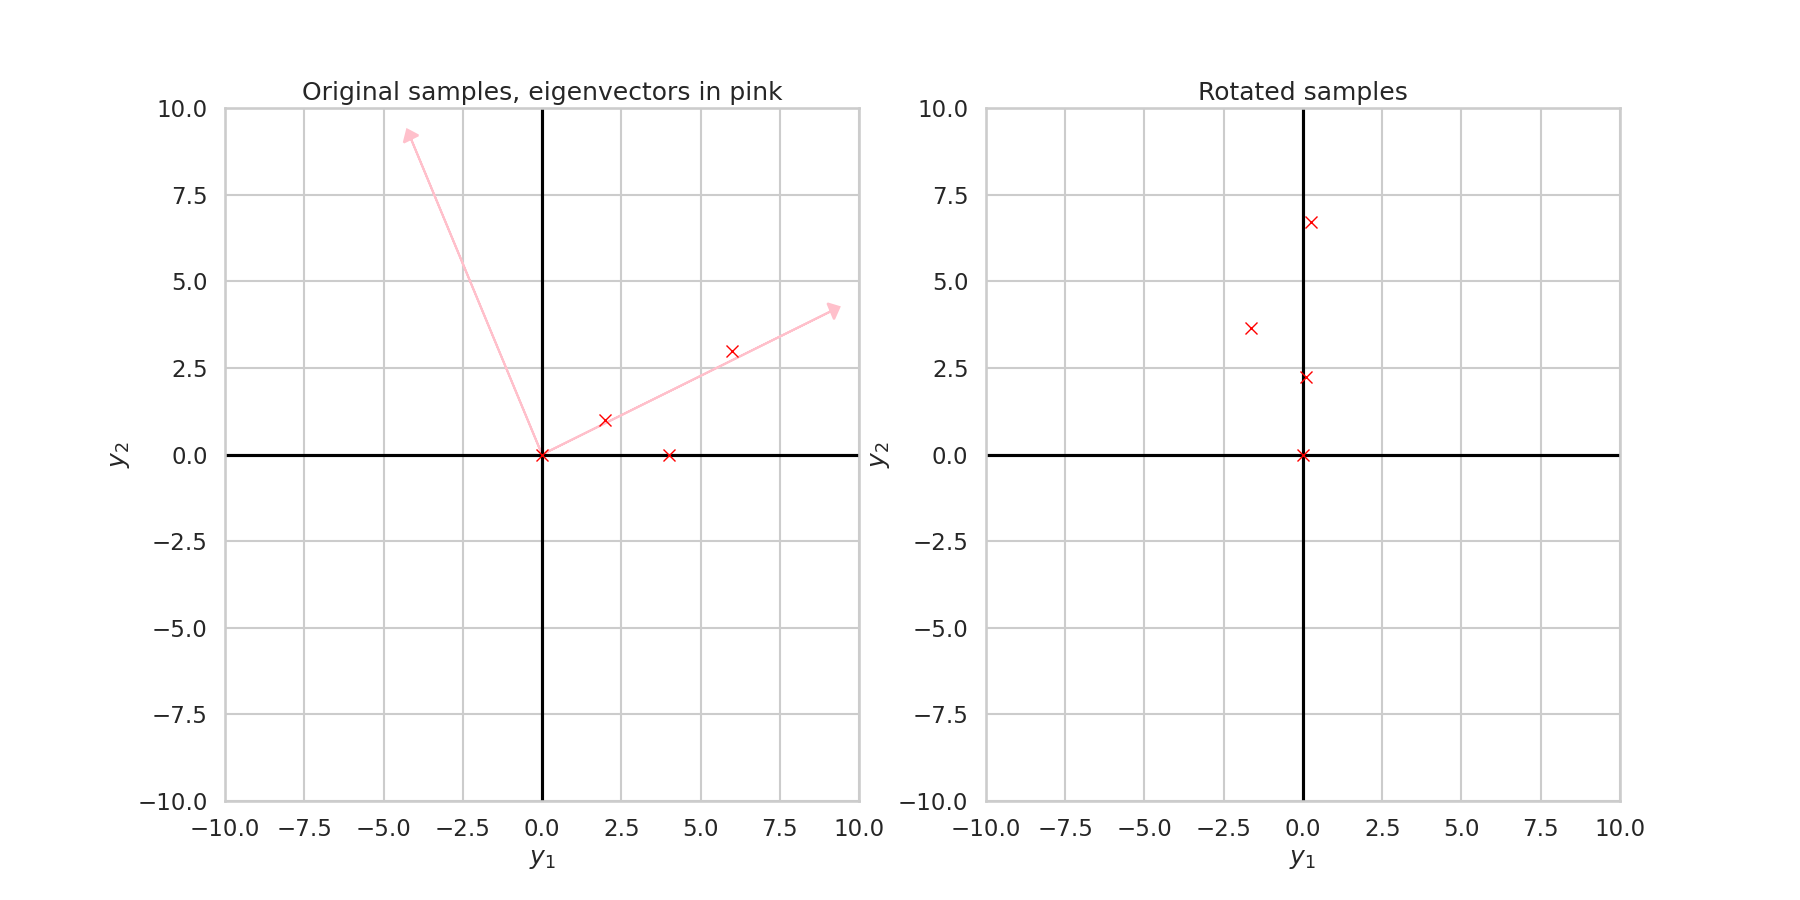
\includegraphics[width=0.68\textwidth]{assets/ex-1/kl-transform.png}
    \label{fig:kl-transform}
  \end{figure}

  When talking about the \textbf{most significant eigenvector}, we can say that it is the
  eigenvector with the \textbf{largest associated eigenvalue}. In this case, we have that $\lambda_1 < \lambda_2$,
  hence the most significant eigenvector is $v_2$. Looking to the plots above we
  can note, as expected, that $v_2$ does look like it "fits the data the best".

  Finally, we could also be interested in mapping the samples onto the dataset's
  \textbf{most significant dimension}: here, we would be interested in the projection
  of the samples onto the eigenvector $v_2$, with the greater eigenvalue. As such,
  we'd only consider the second coordinate of the previously calculated mapped samples,
  which would lead us to the following plot:

  \begin{figure}[h]
    \centering
    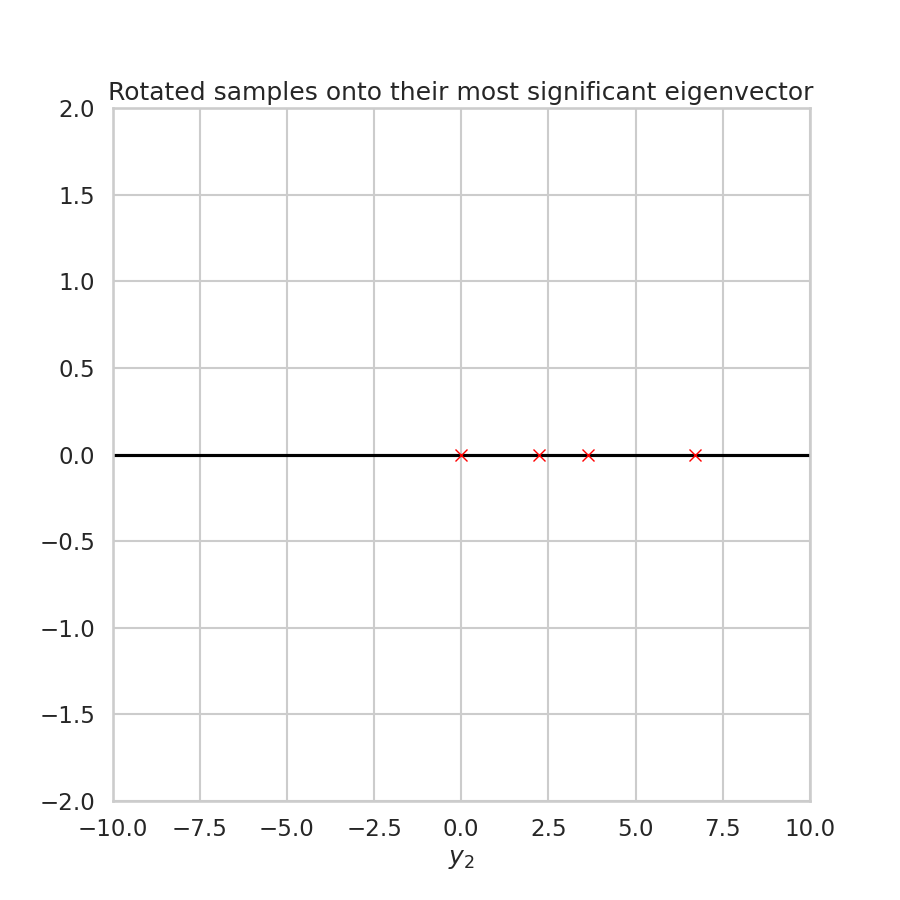
\includegraphics[width=0.4\textwidth]{assets/ex-1/kl-transform-1d.png}
    \label{fig:kl-transform-1d}
  \end{figure}

  \begin{tcolorbox}[enhanced jigsaw,halign=center,colback=bg,boxrule=0pt,arc=1pt]
    \item Given the following datasets where observations are in $\mathbb{R}^2$ and belong
    to one of two classes, which principal components can accurately discriminate
    between the class per dataset?
  \end{tcolorbox}

  \begin{figure}[h]
    \centering
    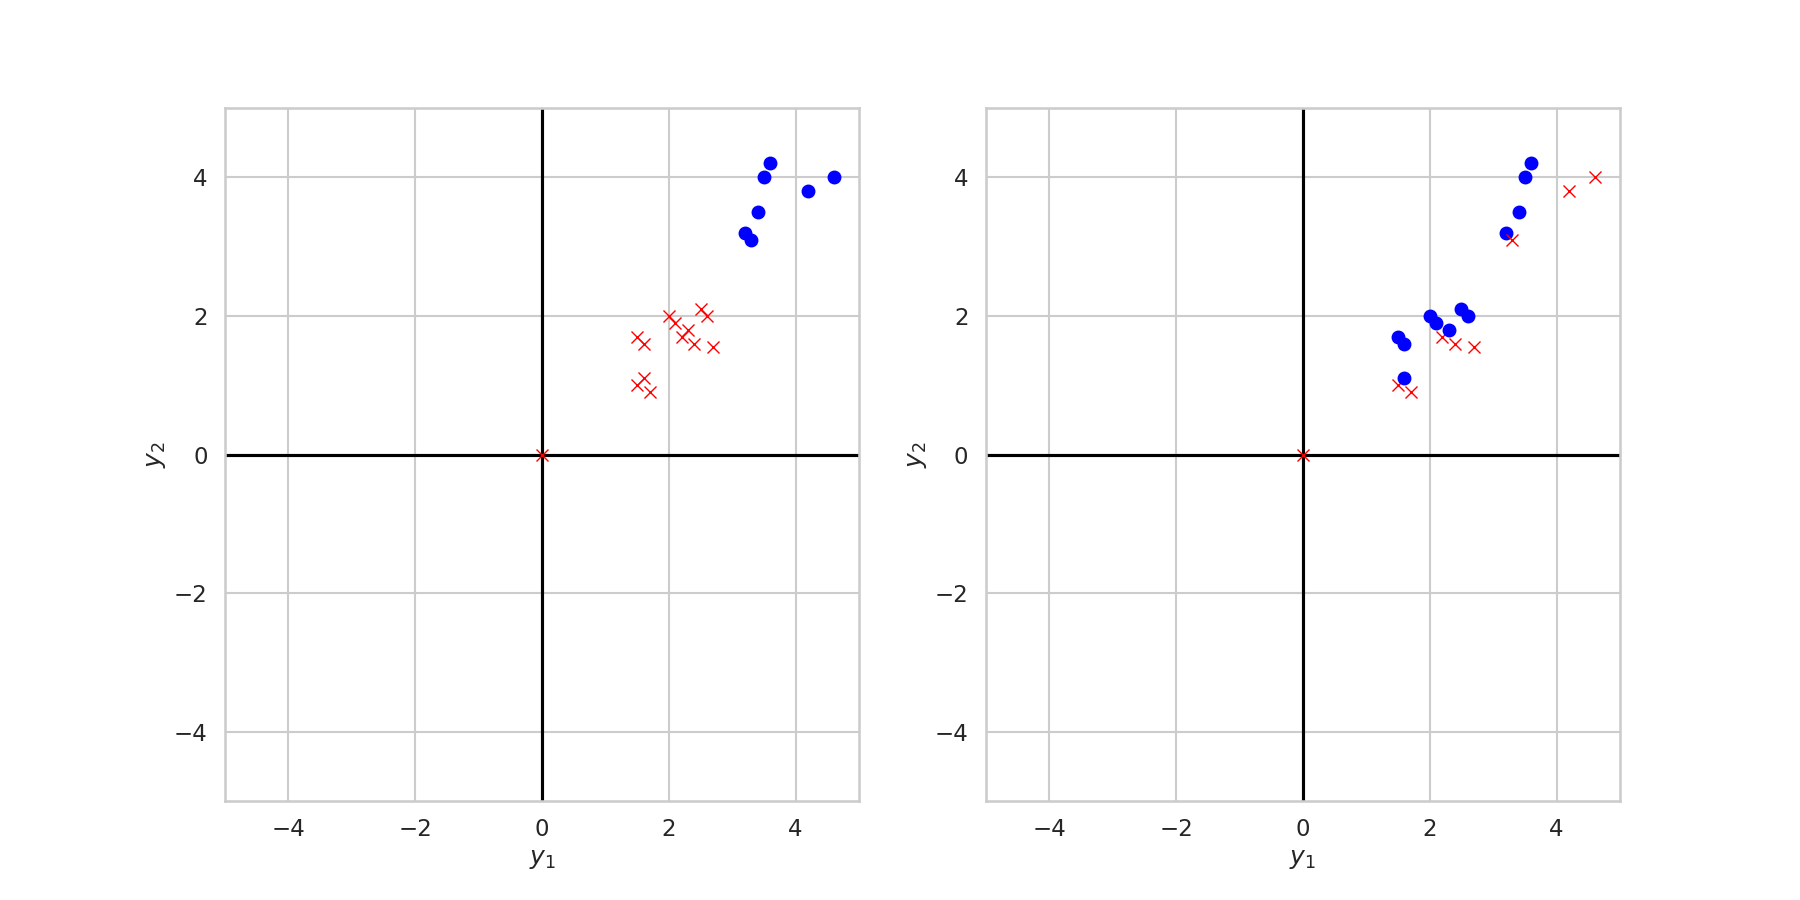
\includegraphics[width=0.8\textwidth]{assets/ex-2/samples.png}
    \label{fig:samples-2}
  \end{figure}

  \textit{Note: the datasets used here are close, but \underline{not equal} to
    the ones used in the original exercise. The logic applied, however, is the same.}

  Eigenvalues are directly related to the variance of the data along the eigenvectors.
  With that said, we can think about this problem as the one of minimizing the
  error along the eigenvectors: specifically, the farther the data is from the
  vector, the more variance, and so on. As such, we associate larger eigenvalues to
  vectors that are more likely to discriminate between the classes, with more
  variance associated. That's not always the case, of course: in data that appears
  to be "mashed together", the eigenvectors may not be able to discriminate between
  the classes (just like in this case). That said, we can still decide whether
  lowest or largest eigenvalues are more likely to discriminate between the classes
  by looking at labeled data:

  \begin{figure}[h]
    \centering
    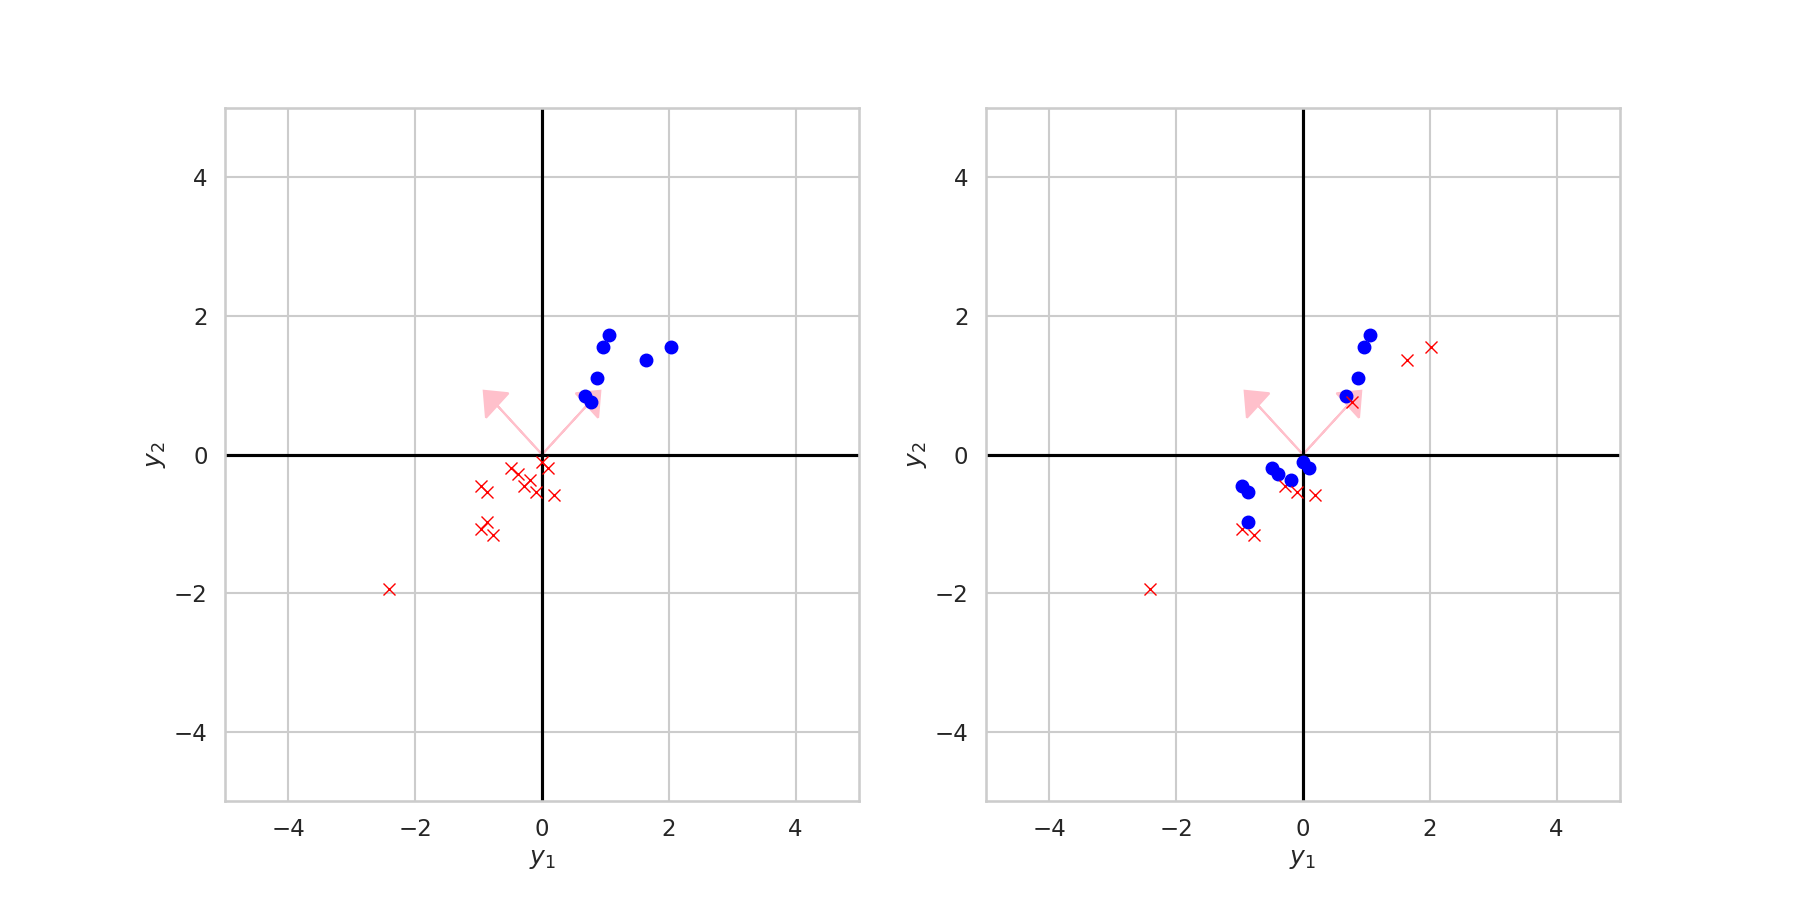
\includegraphics[width=0.8\textwidth]{assets/ex-2/scaled-samples.png}
    \label{fig:samples-2-scaled}
  \end{figure}

  Note that, here, we're now working with scaled data (unit variance and zero mean).
  With that said, with the samples themselves having the same features, only
  labelled differently, we know that their eigenvalues and eigenvectors will be the same.
  As such, we know that in both cases the "largest" and "smallest" eigenvalues will
  be the same.

  Considering $v_1$ as the vector with an $y=x$-ish slope, and $v_2$
  as the vector with an $y=-x$-ish slope, we can see that $v_1$'s eigenvalue must
  be smaller than $v_2$'s, as the former minimizes the distance between itself
  and the samples much more. \textit{This is how we distinguish largest from smallest eigenvalues}.

  With all this gathered, we're now able to assert that the largest eigenvalue,
  associated with $v_2$, best fits the data for the left-most plot, while
  the smallest eigenvalue, associated with $v_1$, best fits the data for the
  right-most plot.

  \begin{tcolorbox}[enhanced jigsaw,halign=center,colback=bg,boxrule=0pt,arc=1pt]
    \item The following top-7 eigenvalues explain 90\% of the variation of dataset $X$:

    \begin{equation*}
      \lambda_1 = 20, \quad \lambda_2 = 10, \quad \lambda_3 = 5, \quad \lambda_4 = 4, \quad \lambda_5 = 3, \quad \lambda_6 = 2, \quad \lambda_7 = 1
    \end{equation*}

    What is the most accurate information regarding $X$?

    \begin{enumerate}
      \item $X$ has less than 7 attributes.
      \item $X$ has 7 attributes.
      \item $X$ has more than 7 attributes.
      \item $X$ has 11 attributes.
    \end{enumerate}
  \end{tcolorbox}

  We know that the proportion of variance explained by a given feature
  is given by the quotient between its eigenvalue and the sum of all
  eigenvalues. In a similar manner, we can say that the $n$ most significant
  features explain the proportion of variance given by the sum of their
  eigenvalues divided by the sum of all eigenvalues. Let's try to decode this exercise:

  \begin{equation*}
    0.9 = \frac{\sum_{i=1}^7 \lambda_i}{\sum_{i=1}^n \lambda_i} = \frac{45}{\sum_{i=1}^n \lambda_i}
  \end{equation*}

  Putting it in another way, an eigenvalue of $45$ would be able to explain
  90\% of the variance of the dataset. As such, we can say that a unit-like
  eigenvalue, $\lambda_k = 1$, would be able to explain 2\% of the variance.
  Considering that the least significant eigenvalue from the top-7 is $1$,
  all other eigenvalues after it would be able to explain, at best, 2\% of the
  variance. As such, we can say that, to explain all the variance in the dataset,
  we'll need \textbf{at least} $7 + \frac{100 - 90}{2} = 12$ features.

  The fourth option is, then, the most accurate one.

  \begin{tcolorbox}[enhanced jigsaw,halign=center,colback=bg,boxrule=0pt,arc=1pt]
    \item Given a set of data points in $\mathbb{R}^3$, the following covariance
    matrix was obtained:

    \begin{equation*}
      \Sigma = \begin{bmatrix}
  6.66667 & 2.66667\\
  2.66667 & 2\\
\end{bmatrix}
    \end{equation*}

    as well as the following eigenvectors retrieved:

    \begin{equation*}
      v_1 = \begin{bmatrix}
  0.707107\\
  -0.707107\\
\end{bmatrix}, \quad v_2 = \begin{bmatrix}
  0.910633\\
  0.413216\\
\end{bmatrix}, \quad v_3 = \begin{bmatrix}
  0.9443\\
  -0.3183\\
  -0.0836\\
\end{bmatrix}
    \end{equation*}

    Please select the more complete answer:

    \begin{enumerate}
      \item eigenvalue $\lambda_1$ is approximately 1626
      \item eigenvalue $\lambda_2$ is approximately 129
      \item eigenvalues $\lambda_1$ and $\lambda_2$ explain > 99\% of the variation in the data
      \item all of the above
    \end{enumerate}
  \end{tcolorbox}

  This is a rather straight forward answer. We must first calculate the
  eigenvalues, of course, from the characteristic polynomial:

  \begin{equation*}
    \det(\Sigma - \lambda I) = 0
  \end{equation*}

  Performing several more \textit{continhas} (which won't be here), we can see that the eigenvalues
  are:

  \begin{equation*}
    \lambda_1 \approx 1626.5, \quad \lambda_2 \approx 129.0, \quad \lambda_3 \approx 7.1
  \end{equation*}

  Therefore, both $a)$ and $b)$ are correct. As for $c)$, we can calculate the proportion of
  variance explained by each eigenvalue, as follows:

  \begin{equation*}
    p_k = \frac{\sum_{i=1}^k \lambda_i}{\sum_{i=1}^n \lambda_i}
  \end{equation*}

  \begin{equation*}
    p_2 = \frac{1626.5 + 129.0}{1626.5 + 129.0 + 7.1} = 0.99597
  \end{equation*}

  We can, therefore, assert that $c)$ is also correct, hence the correct option
  here is $d)$.

  \begin{tcolorbox}[enhanced jigsaw,halign=center,colback=bg,boxrule=0pt,arc=1pt]
    \item Given the following dataset:

    \begin{table}[H]
      \centering
      \begin{tabular}{c|c|c}
              & $y_1$ & $y_2$ \\ \hline
        $x_1$ & 1     & -1    \\
        $x_2$ & 0     & 1     \\
        $x_3$ & -1    & 0
      \end{tabular}
    \end{table}

    and the corresponding eigenvectors and eigenvalues:

    \begin{equation*}
      \begin{aligned}
        \lambda_1 & = \nicefrac{3}{2}, \quad               &  & \lambda_2         = \nicefrac{1}{2} \\
        v_1       & = \begin{bmatrix}
  0.707107\\
  -0.707107\\
\end{bmatrix}, \quad &  & v_2 = \begin{bmatrix}
  0.910633\\
  0.413216\\
\end{bmatrix}
      \end{aligned}
    \end{equation*}

    Transform the input data using PCA.

  \end{tcolorbox}

  Given both eigenvectors, we can, of course, write the transformation matrix
  as:

  \begin{equation*}
    U_{K-L} = \begin{bmatrix}
  0.707107 & 0.707107\\
  -0.707107 & 0.707107\\
\end{bmatrix}
  \end{equation*}

  As it had been stated a few questions ago, the mapping from the original
  axes to the new ones is given by $x' = U_{K-L}^T x$. As such, we can
  rewrite the dataset as:

  \begin{equation*}
    \begin{aligned}
      x_1' & = \begin{bmatrix}
  0.707107 & -0.707107\\
  0.707107 & 0.707107\\
\end{bmatrix} \begin{bmatrix}
  1 & 0 & 0 & 0\\
\end{bmatrix} = \begin{bmatrix}
  1.41421\\
  0\\
\end{bmatrix} \\
      x_2' & = \begin{bmatrix}
  0.707107 & -0.707107\\
  0.707107 & 0.707107\\
\end{bmatrix} \begin{bmatrix}
  0\\
  1\\
\end{bmatrix} = \begin{bmatrix}
  -0.707107\\
  0.707107\\
\end{bmatrix} \\
      x_3' & = \begin{bmatrix}
  0.707107 & -0.707107\\
  0.707107 & 0.707107\\
\end{bmatrix} \begin{bmatrix}
  1 & 1 & 1 & 1\\
\end{bmatrix} = \begin{bmatrix}
  -0.707107\\
  -0.707107\\
\end{bmatrix}
    \end{aligned}
  \end{equation*}

  Below we can see the before and after of the transformation:

  \begin{figure}[h]
    \centering
    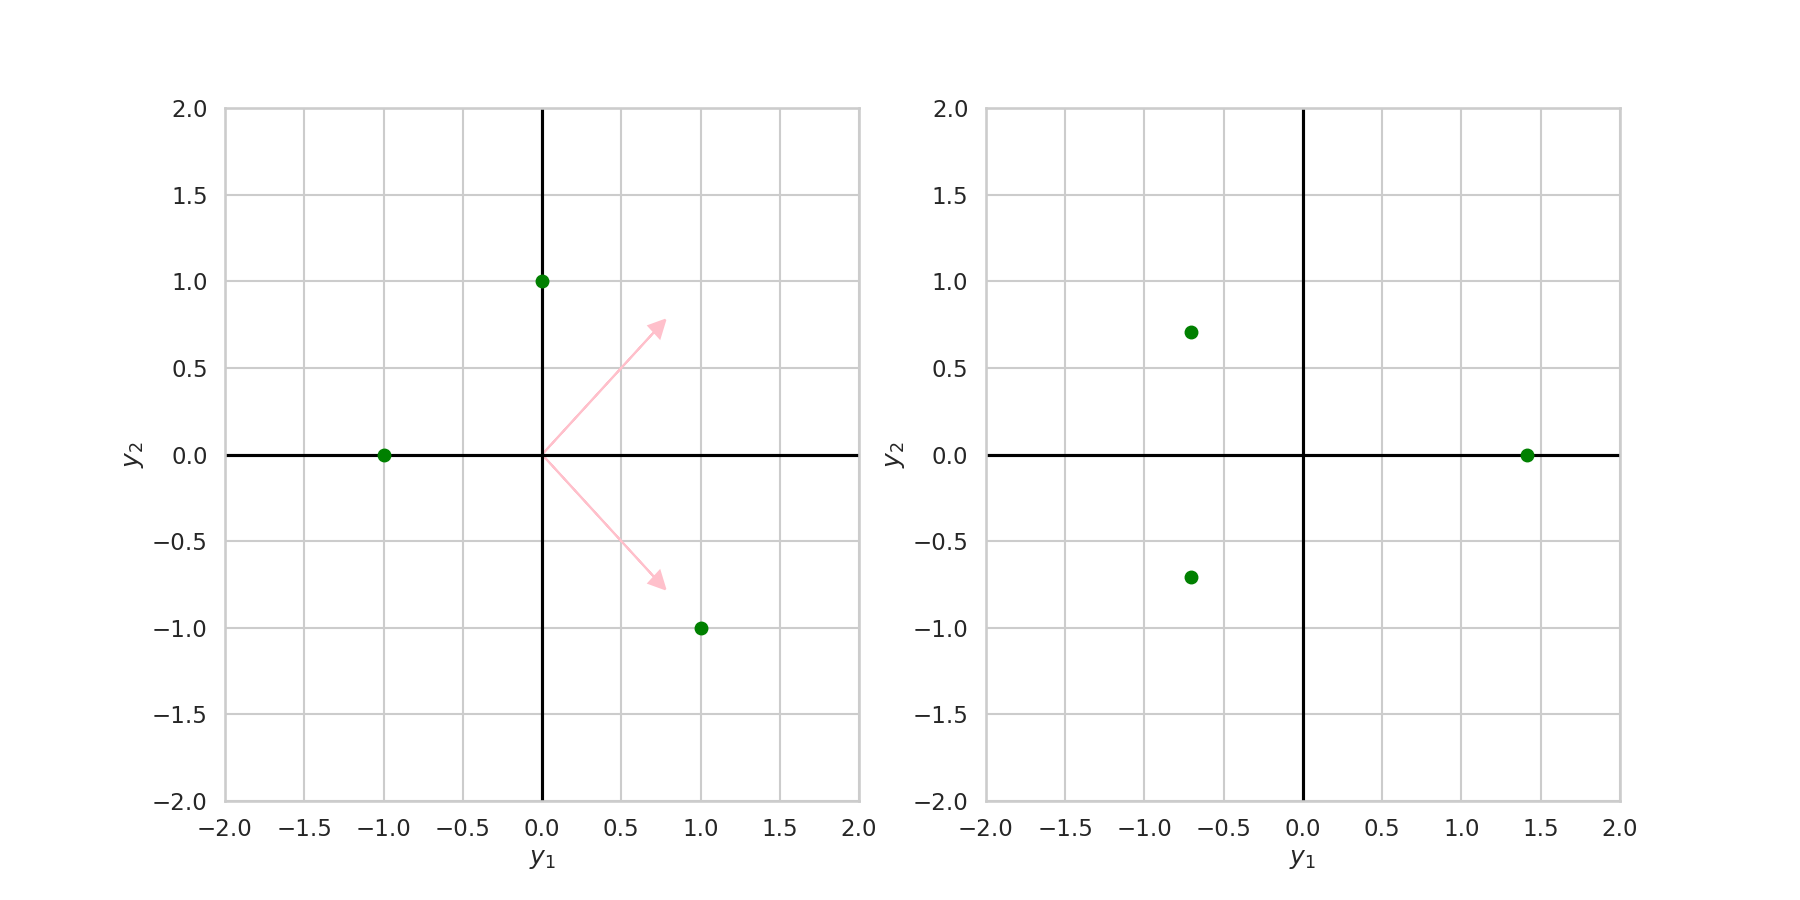
\includegraphics[width=0.75\textwidth]{assets/ex-5/samples.png}
    \label{fig:samples-5}
  \end{figure}

\end{enumerate}

\end{document}
